\cotefile{138}
\scanpage{46}
% archive foliation: 45
Posons pour abréger $X=C_2$, soit $D$ le diviseur de
\unsure{ramfctn|ramification} sur $X$ (de degré 6) -- son corps de
décomposition est $\mathbb Q(i)$; \deleted{posons $X^*=X\setminus D$},
\inserted{$X^*=X\setminus D$}.
\deleted{et soit $\widetilde X^{\unsure{*}}$ le rev. universel abélien de $X^*$}

Soit $X_\infty$ le \inserted{pro-}revêt \deleted{abélien} \inserted{principal} de $X$ défini par
la famille des $\unsure{C_n|\mathcal C_n}$ ($n$ pairs), il a comme
groupe $(\Pi_\infty)_{\deleted{\unsure{X_2}}}$

\scanpage{47}
% archive foliation: 46
\diagram{\begin{tikzcd}[ampersand replacement=\&,row sep=large]
X_n=\unsure{\widehat{\operatorname{Spec}}|\operatorname{Spec}}\,k[x_n]\arrow[d]\\
X_1=\unsure{\widehat{\operatorname{Spec}}|\operatorname{Spec}}\,k[x_1=z]\arrow[d]\\
X_0=\unsure{\widehat{\operatorname{Spec}}|\operatorname{Spec}}\,k[u]
\end{tikzcd}}
\figure{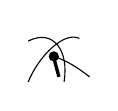
\begin{tikzpicture}[scale=.65]
\draw (-.5,.1) .. controls (0,.35) and (.3,-.1) .. (.2,-.7);
\draw (-.5,-.7) .. controls (-.3,-.2) and (.2,.3) .. (.5,.15);
\draw (0,-.2) .. controls (.3,-.3) and (.5,-.45) .. (.7,-.6);
\fill (0,-.2) circle (.10);\draw[very thick] (0,-.23)--(.1,-.6);
\end{tikzpicture}}
\figure{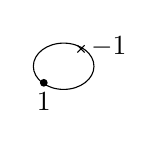
\begin{tikzpicture}[scale=.7]
\draw (0,0) ellipse (.55 and .42);
\fill (-.36,-.30) circle (.07);\node[below] at (-.36,-.30){$1$};
\draw (.25,.38)--(.38,.25) (.25,.25)--(.38,.38);
\node[right] at (.32,.35){$-1$};
\end{tikzpicture}}
\[
\deleted{\unsure{x_n}}\quad x_n^n=x_1
\]
\diagram{\ensuremath{\boxed{\begin{array}{ccc}
n&\left\{\begin{array}{c}1\\1\\\vdots\\1\end{array}\right.&n
\end{array}}}}
\unsure{ramfctn|ramification} au dessus des
$\mathrm{pts}\ 0,\infty$ (où la \unsure{ramfctn|ramification} est $n$)
\unsure{pts} de \unsure{ramfctn|ramification} en haut: $0,\infty$

\diagram{\ensuremath{\boxed{\begin{array}{ccc}2&2&\begin{array}{c}1\\1\end{array}\end{array}}}}
\[
u=\frac12-\frac14(z+z^{-1})
\]
\unsure{ramfctn|ramification} au dessus de

$0$ \deleted{\unsure{pts|pas} \unsure{degrés} (\unsure{pts} au dessus}
\inserted{($z=1$, \unsure{ramfctn|ramification} $2$)}

$1$ ($z=-1$, \unsure{ramfctn|ramification} $2$)

\deleted{\unsure{idem}}

$\infty$ ($0$ et $\infty$ \unsure{ramfctn|ramification} $1$)

\[
\mathbb D_\infty=(\mathbb Z_{/2})\underset{1/2}{\mathord{.}}\mu_\infty
\]
\diagram{\begin{tikzcd}[ampersand replacement=\&,column sep=small,row sep=large]
0\ (n)\arrow[d]\& \&\infty\ (n)\arrow[d]\&1\ (1)\arrow[d,"{\text{\textcircled{\unsure{$n$ fois}}}}"]\&\deleted{\unsure{-1\ (1)}}\arrow[d,draw=none,"{\unsure{\downarrow|-}}" description]\\
0\ (1)\arrow[dr]\&\&\infty\ (1)\arrow[dl]\&1\ (2)\arrow[d,dash]\&-1\ \deleted{\unsure{i\ (n)}}\ (2)\arrow[d]\\
\&\infty\&\&0\&1
\end{tikzcd}}
\margin{$n$ pair}

\figure{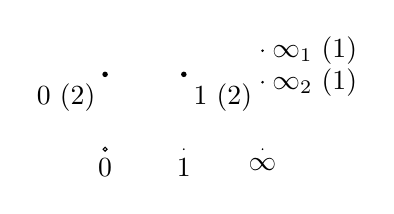
\begin{tikzpicture}
\fill (0,0) circle (.035) node[below left]{$0\ (2)$};
\fill (1,0) circle (.035) node[below right]{$1\ (2)$};
\fill (2,.30) circle (.018) node[right]{$\infty_1\ (1)$};
\fill (2,-.10) circle (.018) node[right]{$\infty_2\ (1)$};
\draw (0,-.95) circle (.025);\node[below] at (0,-.95){$0$};
\fill (1,-.95) circle (.012) node[below]{$1$};
\fill (2,-.95) circle (.012) node[below]{$\infty$};
\end{tikzpicture}}

\figure{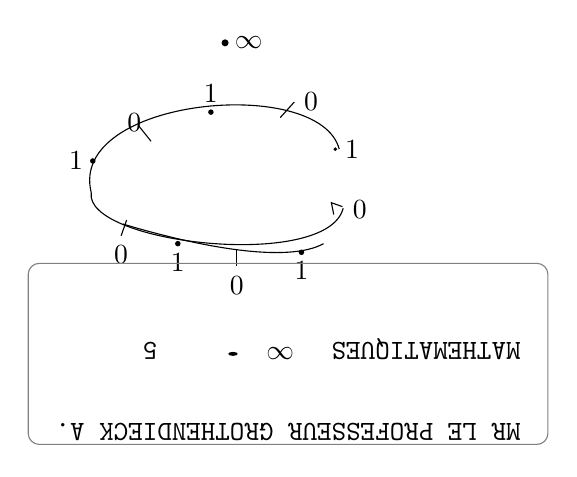
\begin{tikzpicture}[x=1cm,y=1cm]
\fill (0,1.9) circle (.045) node[right]{$\infty$};
\draw (-1.7,0) .. controls (-2,1.2) and (1.2,1.5) .. (1.45,.55);
\draw (-1.7,0) .. controls (-1.8,-.65) and (1.3,-1) .. (1.5,-.2);
\draw (-1.3,-.4) .. controls (-.3,-.7) and (.8,-.9) .. (1.25,-.65);
\fill (-1.68,.4) circle (.035) node[left]{$1$};
\fill (-.18,1.02) circle (.035) node[above]{$1$};
\fill (1.4,.55) circle (.025) node[right]{$1$};
\fill (-.6,-.65) circle (.035) node[below]{$1$};
\fill (.97,-.76) circle (.035) node[below]{$1$};
\draw (-1.1,.85)--(-.94,.65) node[above left]{$0$};
\draw (.7,.95)--(.88,1.15) node[right]{$0$};
\draw (-1.25,-.35)--(-1.32,-.55) node[below]{$0$};
\draw (.15,-.72)--(.15,-.94) node[below]{$0$};
\draw (1.49,-.18)--(1.35,-.13)--(1.38,-.28);\node[right] at (1.5,-.22){$0$};
\draw[gray,rounded corners] (-2.5,-3.2) rectangle (4.1,-.9);
\node[rotate=180,align=left] at (.8,-2.5){\texttt{MR LE PROFESSEUR GROTHENDIECK A.}\\[.6cm]\texttt{MATHEMATIQUES\qquad\qquad\qquad 5}};
\fill (.1,-2.05) ellipse (.06 and .025);\node[right] at (.4,-2.05){$\infty$};
\end{tikzpicture}}

\scanpage{48}
% archive foliation: 47
% The printed sheet is upside down in the supplied scan; reading order below follows its text upright.
ACADEMIE DE MONTPELLIER

\texttt{----------}

JC/JV

LE RECTEUR DE L'ACADEMIE DE MONTPELLIER

Chancelier des Universités

VU\qquad la loi N° 68-978 du 12 novembre 1968
d'orientation de l'enseignement supérieur
et notamment son article 18

VU\qquad la démission présentée par M. le Profes-\\
seur Jacques ROUZAUD, administrateur
provisoire de l'Université de
MONTPELLIER II

A R R E T E

\texttt{-----------}

\uline{Article premier}.

La démission de M. le Professeur Jacques ROUZAUD
de ses fonctions d'administrateur provisoire de
l'Université de Montpellier II est acceptée à compter
du 26 juin 1978 et l'arrêté rectoral du 15 décembre
1977 est abrogé à la même date.

\uline{Article deux.}

Monsieur Yvan MEYERHOEFFER, Conseiller du Tribunal
Administratif de Montpellier, est chargé des fonctions
d'administrateur provisoire de l'Université de
Montpellier II à compter du 27 juin 1978 et jusqu'à
la date d'installation d'un président élu.

Fait à Montpellier, le 27 juin 1978

LE RECTEUR,

\figure{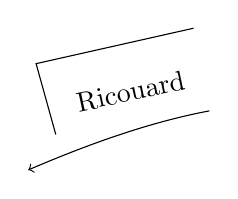
\begin{tikzpicture}[x=1cm,y=1cm]
\node[rotate=12] at (0,0) {\unsure{Ricouard}};
\draw (0.8,0.8)--(-1.2,0.35)--(-0.95,-0.55);
\draw[->] (1.0,-0.25) .. controls (0.2,-0.4) and (-0.6,-0.7) .. (-1.3,-1.0);
\end{tikzpicture}}

\uline{Diffusion} : liste D

n° 4027

MONTPELLIER, le 27 Juin 1978

\scanpage{49}
% archive foliation: 48
\[
z'=z^3
\]
\[
y'=y(y^2-3x^2)
\]
\[
x'=-x(x^2-3y^2)
\]
\[
\begin{aligned}
z^6+y^2(y^4+9x^4-6x^2y^2)+x^2(x^4+9y^4-6x^2y^2)\\
{}=x^6+y^6+z^6+\deleted{\unsure{9}}\inserted{\unsure{3}}x^2y^2(x^2+y^2)
=\deleted{(x^2+y^2+z^2)^3}\\
{}=x^6+y^6+z^6-3x^2y^2z^2
\end{aligned}
\]
\[
\left(\frac yz\right)^2+\left(\frac xz\right)^2=-1
\qquad x^6+y^6+z^6+
\]
$a$ et $b$
\[
\deleted{a^2+b^2=-1}
\]
\[
\deleted{x^2+y^2+z^2}\qquad\deleted{x^6+y^6+3}
\]

\diagram{\begin{tikzcd}[ampersand replacement=\&,column sep=large,row sep=small]
0\arrow[r,bend left=20]\&0\\
X\quad\unsure{2}\&X'\\[-1ex]
1\quad -1\arrow[r,bend right=20]\arrow[r,bend right=8,shorten <=12pt,shorten >=12pt]\&1\\
\infty\arrow[r,bend right=18]\arrow[dd,dash]\&\infty\arrow[dd,"n"]\\
\&\\
{}\&{}
\end{tikzcd}}
\[
\frac{p(x)}{q(x)}=\lambda
\]
\[
p(x)-\lambda q(x)=0
\]
\[
p'(x)-\lambda q'(x)=0
\]
\[
\lambda=\frac{p'}{q'}\qquad p-\frac{p'}{q'}q=0
\]
\[
(x^2)^n=(\unsure{\pm}x^n)^2
\]
\[
\frac{\unsure{a}z^2+bz+c}{z^2}\qquad
\deleted{q'p\unsure{-}}\quad p'q-q'p=0
\]
\[
\deleted{\unsure{a}}\qquad 2z(az^2+bz+c)-
\]

\scanpage{50}
% archive foliation: 49
U N I V E R S I T E

DES SCIENCES ET TECHNIQUES

DU LANGUEDOC

\texttt{------------}

MONTPELLIER, le 8 JUIN 1978

Service de la Scolarité

MR/GJ

Diffusion : Liste H

N°3548

\uline{AVIS DE SOUTENANCE D'UNE THESE DE DOCTORAT D'ETAT}

\uline{Nom et prénom de la candidate} : LINDHEIMER née MONNIER Arlette

\uline{Titre de la thèse} : Contribution à l'étude diffusiométrique des électrolytes dans
des solvants mixtes de constantes diélectriques variables.

\uline{Date, heure et lieu de soutenance prévus} :

1er JUILLET 1978 à 9 Heures 30 mn

Salle de cours n° 2, U.S.T.L.

\uline{Nom du Directeur de thèse} : Monsieur le Professeur B. BRUN

\uline{Désignation du laboratoire où la thèse est préparée} :

Laboratoire des Interactions moléculaires, U.S.T.L.

\uline{Résumé de la thèse} : Les coefficients de diffusion ioniques ont été mesurés à 25°C
pour des électrolytes dissous dans des solvants mixtes dont les constantes diélec-\\
triques prenaient des valeurs différentes :

- soit élevées comme dans les mélanges eau-N-méthylpropionamide,

- soit faibles comme dans les mélanges eau-alcool et eau-éther.

Dans le premier cas, la loi étendue relative au coefficient de
diffusion a été vérifiée jusqu'à 0,2M environ ; dans les autres cas la présence
d'associations ioniques a été mise en évidence et les paramètres d'associations ont
été obtenus dans le cadre du modèle des paires d'ions.

\uline{Durée approximative des recherches ayant abouti à la thèse} : 5 ans

\uline{Noms des Rapporteurs} :

\diagram{\begin{tabular}{ll}
SANFELD A. & Professeur, Chimie Physique, Univ. BRUXELLES\\
TURQ P. & Chargé de Cours, Chimie Physique, Univ. PARIS\\
BRUN B. & Professeur, Chimie Physique, U.S.T.L.
\end{tabular}}

\uline{Composition du jury} :

\diagram{\begin{tabular}{ll}
BRUN B. & Professeur, Chimie Physique, Univ. Sciences et Techn. Languedoc\\
& MONTPELLIER\\
& (Président)\\
SANFELD A. & Professeur, Chimie Physique, Univ. BRUXELLES\\
TURQ P. & Chargé de Cours, Chimie Physique, Univ. PARIS\\
& (Membre extérieur choisi en raison de sa compétence scientifique)\\
GROMB S. & Professeur, Chimie Physique, U.S.T.L.\\
GIRAL L. & Professeur, Chimie Organique,U.S.T.L.\\
& (Membre étranger à la spécialité de la candidate)
\end{tabular}}

Le Secrétaire Général,

\figure{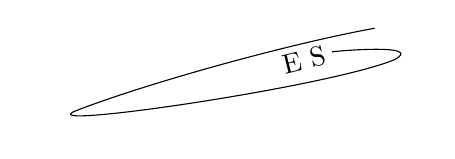
\begin{tikzpicture}
\node[rotate=14] at (1.6,.25){\unsure{E S}};
\draw (2.5,.65) .. controls (1.4,.45) and (-.4,-.05) .. (-1.3,-.4)
.. controls (-1.9,-.65) and (1.9,-.1) .. (2.75,.25)
.. controls (3.15,.46) and (2,.36) .. (1.96,.35);
\end{tikzpicture}}

\uline{E. SIAU}

MR LE PROFESSEUR GROTHENDIECK A.

MATHEMATIQUES\qquad 5

\scanpage{51}
% archive foliation: 50
\[
\cos 2u=\frac{1-\operatorname{tg}^{2}u}{1+\operatorname{tg}^{\unsure{2}}u}
\qquad 2\sin u\cos u=2\text{\uline{$\cos^2u$}}\operatorname{tg}u=
\]
\[
\sin 2u=\frac{2\operatorname{tg}u}{1+\operatorname{tg}^2u}
\qquad
\left\{\begin{aligned}x&=\frac{1-t^2}{1+t^2}\\y&=\frac{2t}{1+t^2}\end{aligned}\right.
\]
\[
t=\frac yx\quad\text{quand }z=1
\]
\[
\deleted{\unsure{1+t^4+2t^2}}
\]
\[
t=0
\]
\[
x=1-t^2\quad y=2t\quad z=1+t^2
\]
\[
\deleted{y\qquad t=\pm i}
\]
\[
\begin{aligned}
z=0\quad\text{i.e. }t=\mp i&\Longrightarrow x=2,\ y=\mp2i\quad
\unsure{\sim|=}\quad x=1\quad y=\mp i\\
&&\unsure{\sim|=}\quad x=\pm i\quad y=1\\
y=0\quad\text{i.e. }t=0&\qquad(1,0,1)
\end{aligned}
\]
\[
x^2+y^2+z^2=0
\]
\diagram{\begin{tikzcd}[ampersand replacement=\&]
C_2=X\arrow[r]\&\mathbb P^1=\widehat{\operatorname{Spec}}(k[t])\\
(\pm i,1,0)\arrow[r]\&t=\mp i\\
(\pm i,0,1)\arrow[r,tail,dash]\&t=0
\end{tikzcd}}
\[
t=\frac yx
\]
\[
\begin{aligned}
x'&=1-t^2=1-\frac{y^2}{x^2}=\frac{x^2-y^2}{x^2}\\
y'&=2t=\frac{2y}{x}\\
z'&=1+t^2=\frac{x^2+y^2}{x^2}
\end{aligned}
\]
ou\quad $(x',y',z')=(x^2-y^2,2xy,x^2+y^2)$
\[
\left\{\begin{aligned}x'&=x^2-y^2\\y'&=2xy\\z'&=x^2+y^2\end{aligned}\right.
\qquad
\begin{aligned}
x'^2+y'^2-z'^2&=x^4+y^4-2x^2y^2\\
&\quad+4x^2y^2\\
&\quad\unsure{-|+}(x^2+y^2)^2=0
\end{aligned}
\]
\diagram{\begin{tikzcd}[ampersand replacement=\&]
X\arrow[r,"2"]\arrow[dr,bend right=20,dash,"f_n"']\&X'\arrow[r,"{n\text{ impair}}"]\&X'\\
\&X\arrow[ur,"2"']\&
\end{tikzcd}}
\[
\deleted{\unsure{t}}\qquad
s=-\frac{t+i}{t-i}=-\frac{(t+i)^2}{t^2+1}
=-\frac{t^2-1}{t^2+1}-\frac{2it}{t^2+1}
\]
\[
\left(\frac{t+i}{t-i}\right)^n\qquad=
\]

\scanpage{52}
% archive foliation: 51
HARVARD UNIVERSITY

DEPARTMENT OF MATHEMATICS

\textsc{Area Code 617}

495--2170

\figure{
\begin{tikzpicture}[scale=.8]
\draw (-.8,1)--(.8,1)--(.8,.35) .. controls (.8,-.25) and (.4,-.65) .. (0,-.9)
.. controls (-.4,-.65) and (-.8,-.25) .. (-.8,.35)--cycle;
\foreach \x/\y/\l/\r in {-.4/.5/V/E,.4/.5/R/I,0/-.25/T/AS}{
\draw (\x-.27,\y-.24) rectangle (\x+.27,\y+.24);
\draw (\x-.3,\y-.2)--(\x-.35,\y-.17)--(\x-.3,\y-.11)--(\x-.3,\y+.1)--(\x-.35,\y+.16)--(\x-.3,\y+.2);
\draw (\x+.3,\y-.2)--(\x+.35,\y-.17)--(\x+.3,\y-.11)--(\x+.3,\y+.1)--(\x+.35,\y+.16)--(\x+.3,\y+.2);
\draw (\x-.23,\y-.2)--(\x-.23,\y+.2)--(\x,\y+.18)--(\x+.23,\y+.2)--(\x+.23,\y-.2)--(\x,\y-.18)--cycle;
\draw (\x,\y+.18)--(\x,\y-.18);
\node[font=\scriptsize,inner sep=0] at (\x-.11,\y){\l};
\node[font=\scriptsize,inner sep=0] at (\x+.11,\y){\r};}
\end{tikzpicture}}

\textsc{Science Center}

\textsc{One Oxford Street}

\textsc{Cambridge, Massachusetts 02138}

June 10, 1978

Dear Friend,

This letter concerns the 80th birthday of Oscar Zariski. This will take place
on April 24th, 1979. I have been talking to Jun-Ichi Igusa, who together with
Jerry Sampson has recently taken over the Editorship of the \uline{American Journal
of Mathematics}, and they agreed that it would be a fine thing to dedicate one
(and perhaps two) issue(s) of the \uline{American Journal} to Oscar on this occasion.
I'm sending this letter out to about thirty of his friends, colleagues and
students to ask if they would like to dedicate a paper to Oscar in this issue.
Unfortunately, as you can guess from the date of his birthday, we can only do
this by adhering to a strict deadline. I sincerely apologize for launching
a project like this at such a late date and must take full blame for this my-\\
self. However, the upshot is that the absolute deadline for contributions
must be November 1st (or January 1st, \uline{if we get enough submissions for a second
issue}): The issue(s) will then be the first one (or first two) of the \uline{American
Journal} in 1979.

I will be very pleased if you find it possible to send me a paper for Oscar's
80th birthday. But I fully understand if the short notice makes this impos-\\
sible. In any case, to help in our planning I would be very grateful if you
would drop me a line now indicating whether or not you expect to be in a posi-\\
tion to send us a manuscript, and, if so, roughly what length it might be.
(We have a maximum of 460 printed pages to use and if we are deluged there is
a small chance that we may have to limit the length of individual submissions.)
Please write me at:

Wallston Road

Tenants Harbor, Maine\quad 04860

U.S.A.

where I will be until about September 10th.

Best regards,

David Mumford/mjm

David Mumford

DM/mjm

\scanpage{53}
% archive foliation: 52
\[
\Pi_n=\mu_n^3/\mu_n
\]
\[
0'\unsure{\leftrightarrow|\leftarrow}0'',\quad
1'\unsure{\leftrightarrow|\leftarrow}1'',\quad
\infty'\unsure{\leftrightarrow|\leftarrow}\infty''
\]
\diagram{\(\begin{array}{ccc}
\underbrace{0'\,\unsure{\leftrightarrow|=}\,1'}&
\underbrace{1'\,\unsure{\leftrightarrow|=}\,\infty'}&?
\end{array}\)}

\diagram{\begin{tikzcd}[ampersand replacement=\&,column sep=small,row sep=large]
\&\&\&\deleted{\unsure{\widetilde X(p,q,r;n)}}
\arrow[dll,"\Pi_n"']
\arrow[dddll,"{\mu_p\times\mu_q\times\mu_r\times\Pi_n}" description]
\arrow[dd,leftrightarrow,"{\mu_p\times\mu_q\times\mu_r}"]
\arrow[dddddll,bend left=80,leftrightarrow,"{\mu_{2p}\times\mu_{2q}\times\mu_{2r}\times\Pi_n}"]\&\\
\&\widetilde X_2(p,q,r)=X_2(2p,2q,2r)\arrow[dd,"{\mu_p\times\mu_q\times\mu_r}"]\&\&\&\\
X_2(p,q,r)\arrow[dddr,"{\mu_p\times\mu_q\times\mu_r}"']\&\&\&\widetilde X_2(n)\arrow[dll,"\Pi_n"']\arrow[d,"\unsure{\mu_2}"]\&\\
\&X_2(2,2,2)=\widetilde X_2\arrow[dr,"\mu_2"]\arrow[dd,"\mu_2^3"']\&\&X_{4n}\arrow[dl,"\Pi_n"]\&\\
\&\&X_4\arrow[dl,"\Pi_2"]\arrow[ddl,bend left=15,"\Pi_4"]\&\&{}\\
\&X_2\arrow[d,"\Pi_2"']\&\&\&\\
\&X_1\arrow[uurrr,bend right=40,dash,"\Pi_{2n}"']\&\&\&
\end{tikzcd}}
\[
\deleted{\unsure{\mu_n\cdot1}}\qquad
\deleted{\unsure{\Pi_n=\mu_n^3/\mu_n}}
\]
\margin{si $p=q=r=1$, $n=2$
on trouve
\[
\mu_2\times\mu_2\times\mu_2\times\underbrace{\Pi_2}_{\mu_2^3/\mu_2}
\]}
\unsure{TSVP}

\scanpage{54}
% archive foliation: 53
\diagram{\begin{tikzcd}[ampersand replacement=\&]
\widetilde X_2\arrow[dr]\&{}\arrow[l,very thick]\&\\
\&X_4\&\unsure{\deleted{R}\inserted{X}|X}_8\arrow[l]
\end{tikzcd}}

% Printed letterhead below is upside down relative to the handwritten diagram.
UNIVERSITÉ DES SCIENCES

ET TECHNIQUES DU LANGUEDOC

\rule{1cm}{.4pt}

INSTITUT DE MATHEMATIQUES

Place Eugène Bataillon

34060 MONTPELLIER CEDEX

\rule{1cm}{.4pt}

Montpellier, le

\scanpage{55}
% archive foliation: 54
\[
X=\frac{y^2-x^2}{z^2}\qquad Y=-\frac{2xy}{z^2}
\]
\[
X+iY=\frac1{z^2}(y^2-x^2-2ixy)=\frac1{z^2}(y\unsure{-|+}ix)^2
\]
\[
\begin{aligned}
(X+iY)^n&=\frac1{z^{2n}}(y-ix)^{2n}
=\frac1{z^{2n}}\bigl(P_n(x,y)+iQ_n(x,y)\bigr)\\
&\overset{?}{=}\frac{y'^2-x'^2}{z'^2}\unsure{-|+}2i\frac{x'y'}{z'^2}
\end{aligned}
\]
$x',y',z'$ fonctions rat. de $x,y,z$ ?? P.ex. $z'=z^n$
\[
\deleted{P_n(x,y)=}\quad\frac{\unsure{A_n}(x,y,z)}{\deleted{z^n}}\quad\text{et}\quad B_n
\]
\[
\unsure{B_n|A_n}(x,y)^2-A_n(x,y)^2=P_n(x,y)
\]
\[
-2A_n(x,y)B_n(x,y)=Q_n(x,y)
\]
\[
X+iY=\left(\frac{y-ix}{z}\right)^2=\left(\frac yz-i\frac xz\right)^2
\]
\[
\left(\frac yz\unsure{-|=}i\frac xz\right.\qquad
\left(\frac yz-i\frac xz\right)^{2n+1}
\]
\margin{$(-i)^3=-i(i^2)=i$}
\[
\left(\frac yz-i\frac xz\right)^3
=\frac1{z^3}\left[
\underbrace{y^3\unsure{-|+}3iy^2x\unsure{-|+}3yx^2+ix^3}_{
\begin{gathered}
y^3-3yx^2+i(x^3-3y^2x)\\
y(y^2-3x^2)+ix(x^2-3y^2)
\end{gathered}}
\right]
\]

\scanpage{56}
% archive foliation: 55
U N I V E R S I T E

DES SCIENCES ET TECHNIQUES

DU LANGUEDOC

\texttt{------------}

MONTPELLIER, le 15 Juin 1978

Service de la Scolarité

MR/GJ

Diffusion : Liste H

N° 3758

\uline{AVIS DE SOUTENANCE D'UNE THESE DE DOCTORAT D'ETAT}

\uline{Nom et prénom du candidat} : WALTER Philippe

\uline{Titre de la thèse} : Recherches écologiques et biologiques sur les Scarabéides Co-\\
prophages d'une savane du Zaïre.

\uline{Date, heure et lieu de soutenance prévus} : 3 JUILLET 1978 à 9 Heures 30 mn

Salle de cours n° 6, U.S.T.L.

\uline{Nom du Directeur de thèse} : Monsieur le Professeur Renaud PAULIAN.

\uline{Désignation du laboratoire où la thèse est préparée} : Zoologie (Professeur LEGENDRE)

\uline{Résumé de la thèse} : Les recherches ont été effectuées sur le Plateau Bateke zaïrois.
Les résultats sont présentés en trois parties :

1) le peuplement (composition d'ensemble, aspects biogéographiques, répartition dans
les différentes formations végétales, fluctuations des densités de population,
sex-ratio)

2) observations autoécologiques et biologiques (préférences trophiques, heures
d'activité, éthologie)

3) morphologie larvaire : description détaillée de 12 larves.

\uline{Durée approximative des recherches ayant abouti à la thèse} : 5 ans 1/2.

\uline{Noms des Rapporteurs} :

\diagram{\begin{tabular}{ll}
PAULIAN R. & , Professeur, Zoogéographie, Rectorat BORDEAUX\\
LAMOTTE M. & , Professeur, Ecologie, Ecole Normale Supérieure PARIS\\
LEGENDRE R. & , Professeur, Zoologie Ecologie, U.S.T.L.
\end{tabular}}

\uline{Composition du jury} :

\diagram{\begin{tabular}{ll}
LEGENDRE R. & , Professeur, Zoologie Ecologie, U.S.T.L.\\
& (Président)\\[1ex]
PAULIAN R. & , Professeur, Zoogéographie, Rectorat BORDEAUX\\
LAMOTTE M. & , Professeur, Ecologie, Ecole Normale Supérieure PARIS\\
& (Membres extérieurs choisis en raison de leur compétence scientifique)\\[1ex]
EUZET L. & , Professeur, Parasitologie, U.S.T.L.\\
& (Membre étranger à la spécialité du candidat)\\
LUMARET J.-P. & , Maître-assistant, Biogéographie, Univ. MONTPELLIER III.\\
BARAUD J. & ., Professeur, Biochimie, Univ. BORDEAUX
\end{tabular}}

Le Secrétaire Général,

\figure{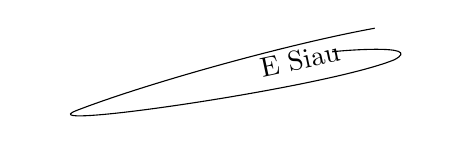
\begin{tikzpicture}
\node[rotate=12] at (1.55,.25){\unsure{E Siau}};
\draw (2.5,.65) .. controls (1.4,.45) and (-.4,-.05) .. (-1.3,-.4)
.. controls (-1.9,-.65) and (1.9,-.1) .. (2.75,.25)
.. controls (3.15,.46) and (2,.36) .. (1.96,.35);
\end{tikzpicture}}

\uline{E. SIAU}

\scanpage{57}
% archive foliation: 56
\unsure{autom.} des

groupoïdes

\scanpage{58}
% archive foliation: 57
\uline{Automorphismes de groupoïdes.}

1) Soient $C$ \deleted{$\unsure{=(C_0,C_1,C_2)}$} un groupoïde,
$C'$ une catégorie, on s'intéresse
à
\[
\operatorname{Hom}(C,C')=\operatorname{Ob}\,\underline{\operatorname{Hom}}(C,C').
\]
On a
\[
\operatorname{Hom}(C,C')\longrightarrow
\operatorname{Hom}(\underbrace{\operatorname{Ob}C}_{C_0},\underbrace{\operatorname{Ob}C'}_{C'_0})
\]
Soit
\[
f_0:C_0\longrightarrow C'_0
\]
on demande les $f:C\unsure{-|\longrightarrow}C'$ qui
lui donnent naissance. On trouve:

\uline{Proposition} a) Pour qu'il existe un
$f$ au dessus de $f_0$, il f. et il s.
que pour $x,y\in C_0$ \unsure{appartenant} à
la \unsure{$=$|même} comp. connexe de $C$
(i.e. tels que $\operatorname{Hom}_C(x,y)\ne\varnothing$) on ait
$f_0(x)\simeq f_0(y)$.
\deleted{b) \unsure{Supposons} cette condition \unsure{satisfaite}.}
b) Pour $\forall$ composante
connexe $C(i)$ de $C$, soit $a_i\in C(i)_0$,
et pour $\forall$ $x\in C(i)_0$, soit
$u_x:a_i\xrightarrow{\sim}x$. Alors
\[
\begin{aligned}
\operatorname{Hom}_{f_0}(C,C')\xrightarrow{\sim}
&\prod_{\unsure{x\in C_0\setminus\{a_i\}}}
\operatorname{Isom}\bigl(f_0(a_{i(x)}),f_0(x)\bigr)\\
&\times\prod_{\unsure{i}}\operatorname{Hom}\bigl(\operatorname{Aut}(a_i),\unsure{\operatorname{Aut}(f_0(a_i))}\bigr)
\end{aligned}
\]

\scanpage{59}
% archive foliation: 58
\[
f\longmapsto\left(
\bigl(\underbrace{\unsure{f_0|f}(u_x)}_{\unsure{\ell_x|e_x}}\bigr)_{x\in C_0},
\bigl(\underbrace{f_{a_i,a_i}:\operatorname{Aut}(a_i)\longrightarrow\operatorname{Aut}(f_0(a_i))}_{\varphi_i}\bigr)
\right).
\]

c) Pour que $f$ soit fidèle, il \unsure{f.|faut} et
suffit que $\forall i\in I$, $\varphi_i$ soit injectif.
Pour que $f$ soit pleinement fidèle,
il \unsure{f.|faut} et suffit que, 1°) pour $i\ne j$,
on ait $\operatorname{Hom}(f_0(a_i),f_0(a_j))=\varnothing$

2°) pour $\unsure{\forall i}\ x,y\in C(i)_0$,
\[
\operatorname{Isom}(f_0(x),f_0(y))\xrightarrow{\sim}\operatorname{Hom}(f_0(x),f_0(y))
\]

3°) $\forall i\in I$, $\varphi_i$ est un iso.

\deleted{d) Si $C$}
Pour que $f$ soit une équivalence,
il f. et s. qu'on ait de plus

4°) Tout $x'\in C'_0$ est isomorphe
à un des $f_0(a_i)$

Pour que $f$ soit un isom.,
il faut et s. qu'on ait 1°, 2°, 3°,
et de plus

4'°) $f_0$ bijective.

\scanpage{60}
% archive foliation: 59
\deleted{
$C=(C_0,C_1)$ groupoïde connexe

$G=\operatorname{Aut}(C)$ gr. des automorphismes

$G^0$ ss gr. des $g\in G$ induisant l'identité sur $C_0$
\diagram{\begin{tikzcd}[ampersand replacement=\&]
1 \arrow[r] \& G^0 \arrow[r] \& G \arrow[r,"{\uuline{\text{Surj}}}"'] \& \unsure{\mathfrak S|\mathcal S}_{C_0} \arrow[r] \& 1
\end{tikzcd}}
[Pour qu'une autoéquivalence \inserted{$u$} soit un iso, il f et s. qu'elle soit bijective sur les objets de $C$, et induise un iso. \deleted{sur les} $\operatorname{Aut}(x)\longrightarrow\operatorname{Aut}(ux)$ pour $\forall x\in C_0$ ; d'autre part, pour toute application $C_0\overset{u_0}{\unsure{-|\longrightarrow}}C'_0$
}
\diagram{\ensuremath{\begin{array}{ccccccccc}
1&-&\operatorname{Aut}^0(C)&-&\operatorname{Aut}C&-&\unsure{\mathfrak S|\mathcal S}_C&-&1
\end{array}}}
\deleted{$\operatorname{Aut}^0(C)\simeq$}

On a
\diagram{\begin{tikzcd}[ampersand replacement=\&,column sep=small]
1 \arrow[r,dash] \& \operatorname{Aut}^0(C,a) \arrow[r,dash] \& \operatorname{Aut}^0(C) \arrow[r] \& \operatorname{Aut}(\underset{\substack{\Vert\\\operatorname{Aut}_C(a)}}{\pi_a}) \arrow[r] \& 1
\end{tikzcd}}
\deleted{\unsure{À}} Pour déterminer \deleted{$\operatorname{Aut}^0(C,a)=$}
\[
\operatorname{Aut}^0(C,a)=\left\{f\in\operatorname{Aut}(C)\ \middle|\ \operatorname{Ob}f=\operatorname{id}\ .\ (f_a:\operatorname{Aut}(a)-\operatorname{Aut}(\underset{\substack{\Vert\\f(a)}}{a}))=\operatorname{id}\right\}
\]
On considère, pour $\forall x\in C_0$,
\[
T_x=\operatorname{Isom}(a,x),\qquad \pi_a\text{-torseur à droite}
\]
et son commutant \deleted{\unsure{\ensuremath{G_x}}} $\operatorname{Aut}(x)$

\scanpage{61}
% archive foliation: 60
\uline{Corollaire} Pour que $f$ soit un iso, il f. et s. que

a) $f$ induit
\[
\pi_0(f):\pi_0(C)\xrightarrow{\sim}\pi_0(C')
\]
b) $f$ \unsure{induise|induit}
\[
\operatorname{Ob}f=f_0:\operatorname{Ob}(C)\simeq\operatorname{Ob}(C')
\]
c) $\forall i\in I$, $f_{a_i,a_i}:\operatorname{Aut}(a_i)\simeq\operatorname{Aut}(f(a_i))$

\margin{\uline{NB} $f$ équivalence $\Longleftrightarrow$ a) et c) sont vrais}

\uline{Corollaire} Pour qu'une application $f_0:C_0\longrightarrow C'_0$ provienne d'un iso $f:C\simeq C'$, il f. et s. que

a) $f_0$ \deleted{\unsure{soit|est}} bijection

b) $f_0$ transforme la relation d'équivalence de $C_0$ (par comp. connexes) en celle de $C'_0$ (condition vide si $C,C'$ connexes).

c) $\forall i\in I$, $\operatorname{Aut}(f_0(a_i))$ est isom. à $\operatorname{Aut}(a_i)$.

\par\hfill\rule{1.5cm}{.4pt}\hfill\par
\deleted{\unsure{On}} Supposons $C=C'$. Alors on trouve
\[
\operatorname{Aut}(C)\longrightarrow\unsure{\mathfrak S|\mathcal S}_{C_0}\qquad\uline{\text{surjection}}
\]
si $\operatorname{Aut}^0(C)$ est le noyau, on trouve donc

\scanpage{62}
% archive foliation: 61
On trouve
\[
\operatorname{Aut}^0(C,a)\simeq\prod_{x\in C_0\setminus\{a\}}\deleted{\unsure{G_x}}\pi_x
\]
\figure{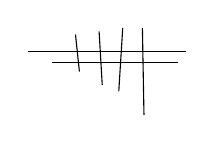
\begin{tikzpicture}[x=1cm,y=1cm]
\draw (0,0)--(2,0) (.3,-.14)--(1.9,-.14);
\draw (.6,.22)--(.65,-.25) (.9,.26)--(.94,-.42) (1.2,.3)--(1.15,-.5) (1.45,.3)--(1.47,-.8);
\end{tikzpicture}}
\deleted{Soit $K$ un graphe}

Soit $I$ un ensemble muni d'une structure polygonale d'ordre $n\geq2$ \deleted{i.e. \unsure{$\Delta_0$}} [pour $n=\unsure{2}$, il faut se donner l'ens. \inserted{de cardinal $2$} des arêtes $\unsure{I^*|I^+}$, \deleted{de} ou ce qui revient au \unsure{$=$|m\textsuperscript{e}}, $\Omega(\Pi)\simeq I\unsure{\wedge|\times}I^*\ldots$ \deleted{cardinal $2$, et}], $\unsure{\mathbb D|D}\ (\simeq\unsure{\mathbb D|D}_n)$ le gr. des autom. de $I$.

Soit $K=K(I)$ le graphe donné par
\diagram{\ensuremath{\begin{array}{ll}
\uline{\text{Sommets}}:&\unsure{\operatorname{Ob}(\Pi)|\Omega(\Pi)}=C_0=\{o,o'\}\\[4pt]
\uline{\text{arêtes}}&\unsure{I^*|I}\quad(\text{indexation }(l_i)_{i\in I})
\end{array}}}
\deleted{\unsure{Toute arête est incidente}}

Incidence : $\unsure{C_0|G_0}\times I$ (\unsure{tte|tt} arête incidente à \unsure{ts|tt} sommets)

\inserted{$G$ opère sur $K(I)$, et on a aussi l'``\uuline{involution}'' $\tau$ qui est l'identité sur $I$, et échange $o,o'$, commutant à $G$.}

\figure{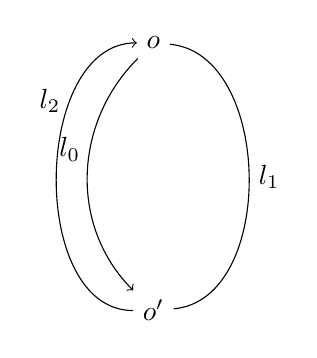
\begin{tikzpicture}[x=1cm,y=1cm]
\node (o) at (0,1.7) {$o$};\node (p) at (0,-1.7) {$o'$};
\draw[->] (p) to[out=180,in=180] node[left,pos=.7] {$l_2$} (o);
\draw[->] (o) to[out=-135,in=135] node[left,pos=.4] {$l_0$} (p);
\draw (o) to[out=-5,in=5] node[right] {$l_1$} (p);
\end{tikzpicture}}
Soit $C(I)$ le groupoïde fondamental de $K(I)$. \deleted{le gr.} $G$ y opère par automorphismes, en opérant transitivement sur $C_0=\{o,o'\}$.

On va regarder le \deleted{commutant}\inserted{normalisateur de $G$} dans

\scanpage{63}
% archive foliation: 62
$G$ dans $\operatorname{Aut}(C(I))$. On a un élément canonique $\tau$

\scanpage{64}
% archive foliation: 63
\diagram{\begingroup
\pgfdeclarelayer{scan064under}
\pgfsetlayers{scan064under,main}
\begin{tikzcd}[ampersand replacement=\&,row sep={1cm,between origins},column sep={1.2cm,between origins},
every matrix/.append style={/tikz/name=scan064matrix},
/tikz/execute at end picture={
\begin{pgfonlayer}{scan064under}
\draw[gray!45,line width=.25pt,arrows=-]
([xshift=-.9cm]scan064matrix-4-1.center)--(scan064matrix-1-3.center)--([xshift=.12cm]scan064matrix-4-5.center)
([xshift=-.9cm]scan064matrix-4-1.center)--([xshift=.12cm]scan064matrix-4-5.center)
([xshift=-.9cm]scan064matrix-4-1.center)--([xshift=1.55cm,yshift=-.2cm]scan064matrix-1-3.center)
(scan064matrix-2-3.center)--([xshift=1cm,yshift=-.35cm]scan064matrix-1-3.center)
(scan064matrix-5-3.center)--([xshift=.15cm]scan064matrix-4-3.center)
(scan064matrix-5-3.center)--([xshift=.25cm]scan064matrix-3-4.center);
\end{pgfonlayer}
}]
\&\& E^+ \arrow[dddll,"p_{20}^+"'] \arrow[d,dashed,"p_{12}^+"'] \arrow[dddrr,"p_{01}^+"] \arrow[ddl,dashed,"\pi_2^+"'] \arrow[ddr,dashed,"\pi_1^+"] \arrow[ddd,"\pi_0^+",near end] \&\& \\[2cm]
\&\& D_{12} \arrow[dl,"\varphi_{21}"'] \arrow[dr,"\varphi_{12}"] \&\& \\
\& S_2 \&\& S_1 \& \\
D_{20} \arrow[ur,"\varphi_{20}"] \arrow[rr,"\varphi_{02}"'] \&\& S_0 \&\& D_{01} \arrow[ul,"\varphi_{10}"'] \arrow[ll,"\varphi_{01}"] \\[2.7cm]
\&\& E^- \arrow[ull,"p_{20}^-"'] \arrow[uuu,dashed,"p_{12}^-",near start] \arrow[urr,"p_{01}^-"] \arrow[uul,dashed,"\pi_2^-"'] \arrow[uur,dashed,"\pi_1^-"] \arrow[u,"\pi_0^-"'] \&\&
\end{tikzcd}\endgroup}
\margin{\deleted{$\unsure{\pi_1^+}$}}
% Faint construction strokes are reproduced on the scan064under layer.
\[
\left\{\begin{aligned}
\rho_0^+&=(p_{01}^+)^{-1}p_{01}^-(p_{20}^-)^{-1}p_{20}^+\\
\rho_{\unsure{0|1}}^+&=(p_{12}^+)^{-1}p_{12}^-(p_{01}^-)^{-1}p_{01}^+\\
\rho_2^+&=(p_{20}^+)^{-1}p_{20}^-(p_{12}^-)^{-1}p_{12}^+
\end{aligned}\right.
\qquad \rho_2^+\rho_1^+\rho_0^+=\operatorname{id}_{E^+}
\]
\[
\begin{aligned}
S_0&\simeq E^+/\rho_0^+\simeq E^-/\rho_0^-\\
S_1&\simeq E^+/\rho_1^+\simeq E^-/\rho_{\unsure{0|1}}^-\\
S_2&\simeq E^+/\rho_2^+\simeq E^-/\rho_2^-
\end{aligned}
\]
\[
\left\{\begin{aligned}
\rho_0^-&=(p_{01}^-)^{-1}p_{01}^+(p_{20}^+)^{-1}p_{20}^-\\
\rho_1^-&=(p_{12}^-)^{-1}p_{12}^+(p_{01}^+)^{-1}p_{01}^-\\
\rho_2^-&=(p_{20}^-)^{-1}p_{20}^+(p_{12}^+)^{-1}p_{12}^-
\end{aligned}\right.
\]

\scanpage{65}
% archive foliation: 64
\margin{\unsure{5.|S.}}
Sous groupes finis de $\operatorname{GP}(1)$ (cas \uline{tame})

\scanpage{66}
% archive foliation: 65
\margin{Cas galoisien $d_{ij}=\deleted{\unsure{N}}d_i=N/\nu_i$}
\[
2-2g'=N(2-2g)\unsure{-}\underbrace{(N\nu\unsure{-|+}\nu')}_{\sum_{i,j}(d_{ij}-1)}
=N(2-2g)-\sum_i\underbrace{\nu_i(N/\nu_i-1)}_{N-\nu_i=N(1-\frac{\nu_i}{N})}
\]
\margin{\deleted{$\unsure{-g'}$}\quad\deleted{\unsure{ici}}}
\[
\boxed{2-2g'=N\left[(2-2g)-\sum_i\left(1-\frac1{d_i}\right)\right]}
\]
Si $g'=0$, on trouve $g=0$ et
\[
\boxed{\frac2N=2-\sum_i\left(1-\frac1{d_i}\right)>0}
\]
d'où
\[
\sum_i\left(1-\frac1{d_i}\right)<2
\]
\uline{Obs} Tous les $d_i\geq2$ \deleted{car} \unsure{ici} $I$ est \uline{\unsure{tout|tjrs}} l'ens de ramification

1) $\operatorname{Card}I=0$\qquad $\dfrac2N=2$, $N=1$ : \deleted{\unsure{par}} $G=1$

2) $\operatorname{Card}I=1$
\[
\frac2N=2-\left(1-\frac1d\right)=1+\frac1d\qquad
2=N+\frac Nd=N+\nu
\]
\margin{or $N\geq1$, $\nu\geq1$\quad donc $N=1$, $\nu=1$\quad $I=\varnothing$}
\uline{impossible}

3) $\operatorname{Card}I=2$
\[
\frac2N=\frac1{d_1}+\frac1{d_2}\qquad
2=\frac N{d_1}+\frac N{d_2}=\nu_1+\nu_2\qquad
\nu_1,\nu_2\geq1\qquad\nu_1=\nu_2=1
\]
\[
d_1=d_2=N\qquad\uline{N\text{ quelconque}}
\]
4) $\operatorname{Card}I=3$
\[
\deleted{\unsure{\frac2N=2}}\qquad
\frac1{\unsure{p|d_1}}+\frac1{\unsure{q|d_2}}+\frac1{\unsure{r|d_3}}>1
\qquad\left(\frac2N=\left(\frac1p+\frac1q+\frac1r-1\right)\right)
\]
OPS\qquad $p\geq q\geq r$

a) $\unsure{r|p}=2$\qquad $\dfrac1p+\dfrac1q>\dfrac12$\qquad i.e. pour $p=\alpha+2$, $q=\beta+2$\quad $(\alpha\geq\beta\geq0$
\margin{$\unsure{\alpha}$}
\[
2p+2q-pq>0\qquad\deleted{\unsure{2(\alpha+\beta)+8-}}
\]
\[
\underbrace{2(\alpha+2)+2(\beta+2)-(\alpha+2)(\beta+2)}_{4-\alpha\beta>0}>0
\]
\[
\alpha\beta<4\qquad
\begin{array}{l}
\beta=0,\ \alpha\text{ quelc.}\\
\beta=1,\ \alpha=1,2,3\\
\deleted{\unsure{\beta=2,\alpha}}
\end{array}
\]
\diagram{\ensuremath{\left\{\begin{array}{lll}
(2,2,p)&p\geq2\text{ quelc.}&N=2p\\
(2,3,3)&&N=12\\
(2,3,4)&&N=24\\
(2,3,5)&&N=60
\end{array}\right.}}
b) $r\geq3$\qquad $\dfrac1p+\dfrac1q>1-\dfrac1r\geq\dfrac23$\quad\uline{impossible} car $\dfrac1p,\dfrac1q\leq\dfrac13$

5) $\operatorname{Card}I\geq4$\qquad $\deleted{\unsure{\sum}}\quad\dfrac1p+\dfrac1q+\dfrac1r+\dfrac1s>2$\qquad $\deleted{\unsure{si}}\ p\geq q\geq r\ \deleted{\unsure{ou}}\geq s$

Faisons d'abord $\operatorname{Card}I=4$
\[
\deleted{\frac1p+\frac1q+\frac1r>2-\frac1s=1+\left(1-\frac1s\right)\geq1+\left(1-\frac1p\right)>1}
\]

\scanpage{67}
% archive foliation: 66
\diagram{\begin{tabular}{c l}
U N I V E R S I T E & Montpellier, le 28 Juin 1978\\
DES SCIENCES ET TECHNIQUES &\\
DU LANGUEDOC &\\
\texttt{------------}&\\
Service de la Scolarité &\\
MR / GJ &\\
Diffusion : Liste A &\\
N° : 4066 &
\end{tabular}}
\uline{AVIS DE SOUTENANCE D'UNE THESE DE DOCTORAT DE 3ème CYCLE}

\uline{( CHIMIE ORGANIQUE PHYSIQUE )}

\uline{Nom et prénom du candidat} :\qquad AURELLY Michèle

\uline{Titre de la thèse} : Application de la corrélation de Hammett à l'étude de l'énolisation des cétones en milieux basique et superbasique.

\uline{Date, heure et lieu de soutenance prévus} :

JEUDI 13 JUILLET 1978 à 16 Heures\\
Salle de cours n° 9 - U. S. T. L.

\uline{Nom du Directeur de thèse} :

Monsieur le Professeur LAMATY.

\uline{Désignation du laboratoire où la thèse est préparée} :

Laboratoire de Chimie Organique Physique.

\uline{Analyse de l'ouvrage} :

Ce travail consiste à cerner de plus près les mécanismes de l'énolisation des cétones par l'étude d'acétophénones et de méthyl-2 phényl-1 butanones-1 substituées, dans des milieux basiques. Les constantes p de Hammett ont été mesurées en fonction de la nature du milieu.

\uline{Durée approximative des recherches ayant abouti à la thèse : 3 ans.}

\uline{Composition du jury proposé} :
\diagram{\begin{tabular}{ll}
MM. : & LAMATY, Président\\
& SCHUE\\
& WYLDE\\
& MION
\end{tabular}}
Le Secrétaire Général,

\figure{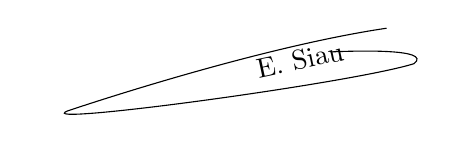
\begin{tikzpicture}[x=1cm,y=1cm]
\node[rotate=12] at (1.55,.25){\unsure{E. Siau}};
\draw (2.65,.65) .. controls (1.3,.45) and (-.5,-.1) .. (-1.4,-.4)
.. controls (-1.9,-.6) and (2.2,-.05) .. (3,.2)
.. controls (3.25,.4) and (2.2,.36) .. (1.96,.35);
\end{tikzpicture}}

\uline{E. SIAU}

\scanpage{68}
% archive foliation: 67
\deleted{
$(p,q,r)$ doit être parmi les \deleted{\unsure{trois}} syst. énumérés

a) $p,2,2$ : $\dfrac1p+\dfrac12+\dfrac12>\left(1+\left(1-\dfrac1s\right)\right)$\quad i.e. $\dfrac1p+\dfrac1s>1$ impossible car $\dfrac1p,\dfrac1s\leq\dfrac12$

b) $(p,3,2)$\quad $(p=3,4,5)$, $s\geq p$ \deleted{\unsure{\ensuremath{\frac1p+\frac13+\frac12}}}
\[
\frac1s+\frac1p+\underbrace{\frac13+\frac12}_{5/6}>2\qquad
\frac1s+\frac1p>\frac76\qquad\text{impossible car }\frac1s,\frac1p\leq\frac13
\]
}
\[
\frac1p+\frac1q>2-\underbrace{\left(\frac1r+\frac1s\right)}_{\substack{\leq1\\\text{car }\frac1r\leq\frac12\\\frac1s\leq\frac12}}\geq1
\quad\text{donc}\quad\frac1p+\frac1q\geq1\quad\text{impossible car }\frac1p,\frac1q\leq\frac12
\]
\uline{Impossible} !

Car si $\operatorname{Card}I\geq4$, on aura
\[
\frac1{d_1}+\frac1{d_2}+\frac1{d_3}+\frac1{d_4}
\deleted{\unsure{+\sum_{5\leq i\leq\nu}\frac1{d_i}}}
>2+\sum_{5\leq i\leq\nu}\left(1-\frac1{d_i}\right)
\underset{2}{\unsure{\vee|\geq}}
\]
et on vient de voir que c'est impossible !

\deleted{
\uline{Étude du cas} \deleted{$\operatorname{Card}I=2$}\inserted{$(N,N)$} : En caractéristique $0$, c'est le cas bien connu
\[
G\simeq\mu_N(k)\simeq\mathbb Z/N\mathbb Z
\]
\deleted{\unsure{Plus gén\textsuperscript{t}|Plus généralement}} \unsure{gén.|Bien}, il en est ainsi si car. $p$ premier à $N$.

Si $p\mid N$, on trouve une $p$-extension \inserted{(de degré $p^r$, tlt ramifiée et \unsure{inséparable})} d'une $N'$-extension kummérienne $(N=p^rN',\ (p,N')=1)$. C'est donc une \uline{extension} \deleted{et} \uline{résoluble}, \inserted{mais mieux :} \deleted{\unsure{On ne peut être plus précis},} \deleted{de} \inserted{les $p$-\deleted{extensions} \unsure{sous-}}

\inserted{\unsure{groupes} $H$ de $\operatorname{GP}(1,k)$ sont \uline{abéliens} et contenus dans}
\deleted{\unsure{toute hypothèse|toute la théorie}. \unsure{On déduit même que l'extension est}}
\deleted{\uline{abélienne finie}}
sous-groupe unipotent de dim $1$, \inserted{conjugués entre eux, et $H$ isom : $(\mathbb Z/p\mathbb Z)^{\unsure{\nu|r}}$.} On trouve donc

$G\subset\text{Borel}$, et par suite $G$ produit $\frac12$ direct d'un groupe cyclique premier à \unsure{$2$|$p$} car., par un $(\mathbb Z/p\mathbb Z)^r$. En fait, on voit aisément (\deleted{\unsure{ici encore}} qu'on est ds le cas précédent (cyclique premier à car., donc kummérien, qui en est exclu), on \unsure{tombe} en contradiction.

\margin{En tous les cas, on a une extension abélienne, \unsure{non kummérienne|kummérienne} (d'ordre premier à $p$) \unsure{sous} \deleted{\unsure{gr.}} \unsure{gr.} $(\mathbb Z/p^r\mathbb Z)^\nu$}

\uline{Étude du cas} $(N,2,2)$, $(\#G=2N)$. En car. $\ne2$, \uline{l'indice}\inserted{\unsure{d'un pt}} de ramification $2$ est ramification modérée, et faisant une \deleted{\unsure{différence}} extension kummérienne de degré $2$, on \deleted{\unsure{tr}} trouve un $X'/Y'$ qui n'a plus que $2$ pts de ramification \deleted{\unsure{dans}} $Y'$, donc $X'/Y'$ est justiciable de l'étude précédente mais \deleted{\unsure{il faut justifier que|il faut vérifier que}}\inserted{\unsure{voir pour|voir}} si $X'$ de genre $0$ (facile)
\diagram{\begin{tikzcd}[ampersand replacement=\&]
X \arrow[d] \& X' \arrow[l] \arrow[d,dash]\\
Y \& Y' \arrow[l]
\end{tikzcd}}
}

\scanpage{69}
% archive foliation: 68
\diagram{\begin{tabular}{cl}
U N I V E R S I T E & Montpellier, le 26 Juin 1978\\
DES SCIENCES ET TECHNIQUES &\\
DU LANGUEDOC &\\
\texttt{------------}&\\
Service de la Scolarité &\\
MR/GJ &\\
Diffusion : Liste A &\\
N°:4000 &
\end{tabular}}
\uline{AVIS DE SOUTENANCE D'UNE THESE DE DOCTORAT D'UNIVERSITE}

\uline{Nom et prénom du candidat} : PAYEN Jean-Luc

\uline{Titre de la thèse} : Contribution à l'étude de la protection des surfaces métalliques par les composés oxyfluorés du phosphore V.

\uline{Date, heure et lieu de soutenance prévus} :

13 JUILLET 1978 à 11 Heures\\
Ecole Nationale Supérieure de Chimie.

\uline{Nom du Directeur de thèse} :

Monsieur le Professeur L. COT.

\uline{Désignation du laboratoire où la thèse est préparée} :\\
Laboratoire de Chimie minérale appliquée - Chimie des Matériaux, E. N. S. C. M.

\uline{Analyse de l'ouvrage} :

Les sels de l'anion $\mathrm{PO3F}^{2-}$ peuvent être utilisés lors de l'opé-\\
ration de post-traitement après phosphatation en substitution des sels de chrome VI hautement toxiques.

Une étude de la nature de la surface crée par phosphatation et passivation par K2PO3F a été entreprise par différentes techniques : ESCA,Microscopies électronique , et ionique. Elle montre une réorganisation physico chimique de la couche.

\uline{Durée approximative des recherches ayant abouti à la thèse} : 2 ans

\uline{Composition du jury proposé} :
\diagram{\begin{tabular}{lll}
MM. & : &\\
&M.&MAURIN\\
&L.&COT\\
&P.&DESRE\\
&J.&DURAND\\
&X.&GRANDIN DE L'EPREVIER\\
&B.&PARANT\\
&P.R&PHILIP
\end{tabular}}
Le Secrétaire Général,

\figure{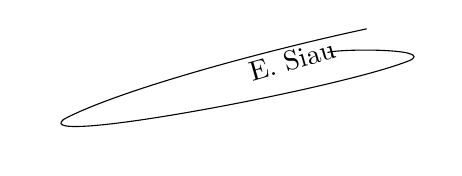
\begin{tikzpicture}[x=1cm,y=1cm]
\node[rotate=16] at (1.55,.3){\unsure{E. Siau}};
\draw (2.5,.7) .. controls (1.1,.4) and (-.7,-.1) .. (-1.35,-.45)
.. controls (-1.8,-.8) and (2.2,-.05) .. (3.05,.3)
.. controls (3.35,.45) and (2.2,.45) .. (2,.4);
\end{tikzpicture}}

\uline{E. SIAU}

\scanpage{70}
% archive foliation: 69
Paradigme \deleted{\unsure{topologique}}\inserted{``gruppentheoretisch''}\\
des surfaces compactes\\
à opérateurs

\scanpage{71}
% archive foliation: 70
Paradigme des courbes algébriques

I\quad Point de vue topologique.

On considère des surfaces topologiques (sans bord) orientables paracompactes \inserted{$X$} -- on se donne aussi un ensemble $\omega$ de cardinal $2$, et on pose
\[
T=\mathbb Z\wedge_{\mathbb Z/2}\omega,
\]
et on suppose donné pour $X$ une $\omega$-orien-\\
tation, i.e. une \inserted{$\mathbb Z/2$-}application \deleted{\unsure{compatible}}\inserted{de $\omega$ dans} l'ens des orientations de $X$, ou ce qui revient au $=$, un isomorphisme du faisceau des entiers tordus sur $X$ avec le faisceau constant $T_X$. On suppose que les composantes connexes $X_i$ de $X$ \deleted{sont}\inserted{est} homéomorphes à un $\widehat X_i\setminus S_i$, où $\widehat X_i$ est une surface compacte, et $S_i$ une partie finie de $\widehat X_i$. On sait que $(\widehat X_i,S_i)$ est détermi-\\
né à isom unique près par $\unsure{X|X_i}$.

(comme le \unsure{décomp.} des compactifiés de Čech

\scanpage{72}
% archive foliation: 71
de $X_i$ suivant les points à l'infini\ldots).

Cl. que $\widehat X_i$ est automatiquement $\omega$-orienté, donc aussi
\[
\widehat X=\coprod\widehat X_i
\]
De cette façon, la catégorie envisagée (des surfaces topologiques ``spéciales'' $\omega$-orientées \inserted{avec homéomorphismes $\omega$-orientés}) devient équivalente à celle des surfaces topologiques \inserted{$\omega$-orientées} à comp. conn. compactes \uline{munies} d'une partie \deleted{\unsure{f}} $S$ discrète, avec les isom. de couples $(\widehat X,S)$.

De $\overline{\mathrm m}$, la catégorie des couples \deleted{$\unsure{(X,S)|(X,o,S)}$} $(X,o,\unsure{\mathcal J|J})$ avec $(X,o)$ comme dessus ($o$ la $\omega$-orientation) et $\mathcal J$ partie discrète de $X$, est équiva-\\
lente à celle des systèmes $(\widehat X,o,S,\mathcal J)$, où $(\widehat X,o)$ est une surface $\omega$-orientée à comp. conn. compactes,

\scanpage{73}
% archive foliation: 72
et $S,\mathcal J$ sont deux parties discrètes disjointes de $\widehat X$.

On va \deleted{\unsure{se}} passer aux catégories isotopiques correspondantes, et en donner des interprétations en termes de théorie des groupes. Bien entendu, pour cette description, on est ramené au cas connexe. On peut \deleted{aussi} noter tt de suite que pour ce pb, on est ramené au cas où $\mathcal J=\varnothing$ [en \deleted{remplaçant}\inserted{\unsure{décrivant|donnant}} dans le cas général comme celui de la donnée d'un $(\widehat X,I)$ \uline{plus} la donnée d'une partie $\mathcal J$ de $I$]. Mais on gardera le pb \unsure{ss|sous} \inserted{la} forme générale, en gardant également la dissymétrie dans le rôle de $S,\mathcal J$ -- mais

\scanpage{74}
% archive foliation: 73
on devra expliciter dans le paradigme
le passage d'une description à
l'autre.

\deleted{La description \unsure{$S\ne\varnothing$}}

1) Cas $\mathcal J=\varnothing$. On va supposer, pour
notre description, que l'on n'est
pas dans les cas $g=0$, $\nu=0,1$
($g=$ genre de $\widehat X$, $S=\operatorname{Card}\nu$)
On associe à $(\widehat X,\widehat o,S)$ \inserted{$(\leadsto)(X,o)$} le
groupe fondamental $\Pi=\pi_1(X)$, considéré
comme groupe extérieur, mais
muni de \unsure{sa|ses} $T$-\unsure{structures|structure} :
locales indexées par $S$, i.e. une
\deleted{famille}\inserted{application}
\[
S\longrightarrow\operatorname{Homext}(T,\Pi)
\]
\deleted{$\unsure{(\varphi_s)_{s\in S}}$}
\inserted{\textcircled{\unsure{$4^\circ$|$1^\circ$}} (Ceci permet
\deleted{$\unsure{\varphi_s\in\Pi}$} de définir
$\Pi_{\unsure{\wedge|1}}\ (\simeq\pi_1(\widehat X))$ comme
groupe quo. de $\Pi$ par le sous-groupe inv. engendré par les
$T\longrightarrow\Pi$.
Si $\nu=0$ i.e. $S=\varnothing$ il faut de
plus \unsure{en} donner un iso
$T\longrightarrow[(\unsure{\bigwedge^2\Pi_{\wedge\mathrm{ab}}})^\vee]$
\unsure{qui} \unsure{de} $T$. \unsure{ou une forme}
i.e. \unsure{primitive} \unsure{sur}
\unsure{le groupe} \unsure{du} \unsure{dual} \unsure{ext.}
de \deleted{$\unsure{\Pi}$} $\unsure{\Pi_\wedge}$.)}
Ceci donne \inserted{\textcircled{$=$}} une description
$1$-isotopique, et $=$ $\infty$-isotopique,
sauf si $g=0$, $\nu=2$ et $g=1$, $\nu=0$,
où les composantes neutres

\scanpage{75}
% archive foliation: 74
du groupe des autom. de $(X,o)$
n'est pas contractible (mais un
$K(\mathbb Z,1)$ resp. un $K(\mathbb Z^{\unsure{2}},1)\ldots$)

$2^\circ)$ $\mathcal J\ne\varnothing$. On a une description
plus jolie (tjrs exception faite
des cas $g=0$, $\nu=0,1$) par le
groupoïde fondamental de $X$
en $\mathcal J$, mais avec $T$-structure
\unsure{à bouts|à bout} sur le groupe extérieur
$\Pi$ associé --- et si $\nu=0$, à la place de
cette structure, il faut donner
\[
T\overset{\unsure{\sim}}{\longrightarrow}
(\bigwedge^2\Pi_{\wedge\mathrm{ab}})^\vee
\]
comme dans $1^\circ\ldots$. Ici on trouve
une description $\unsure{\infty}$-isotopique, même
dans les cas $g=0$, $\nu=2$, ou $g=1$, $\nu=0$.
\margin{vérifier}

\scanpage{76}
% archive foliation: 75
\unsure{groupes} \unsure{prolibres|problèmes}
spéciaux

\scanpage{77}
% archive foliation: 76
\diagram{\begin{tikzcd}[ampersand replacement=\&,column sep=small]
\& R\arrow[dl,"p"']\arrow[d,bend right=15,"q'"']\arrow[d,bend left=15,"q''"]\arrow[dr,"r"]\&\\
S\&A\&F
\end{tikzcd}}
\diagram{\begin{tikzcd}[ampersand replacement=\&,column sep=large]
\& R^\circ=R\arrow[dl,"p^\circ=p"']\arrow[d,bend right=15,"q'{}^\circ=q''"']\arrow[d,bend left=15,"{q''{}^\circ=\deleted{\unsure{q'}}\inserted{q'\circ\sigma_2}}"]\arrow[dr,"{\unsure{q|r}^\circ=\unsure{q|r}\circ\sigma_2}"]\&\\
S\&A\&F
\end{tikzcd}}

\figure{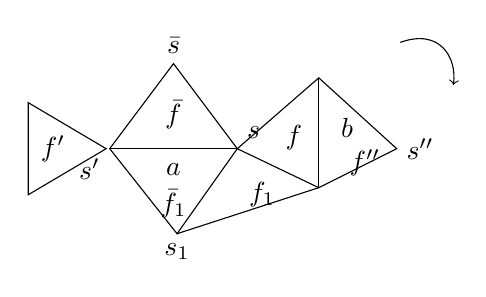
\begin{tikzpicture}[scale=.9]
\draw (-3.1,-.65)--(-3.1,.65)--(-2,0)--cycle;
\draw (-1.95,0)--(-1.05,1.2)--(-.15,0)--(-1,-1.2)--cycle;
\draw (-1.95,0)--(-.15,0);
\draw (-.15,0)--(1,1)--(2.1,0)--(1,-.55)--cycle;
\draw (1,1)--(1,-.55);
\draw (-1,-1.2)--(1,-.55);
\node at (-2.75,0) {$f'$};
\node[below left] at (-1.95,0) {$s'$};
\node[above right] at (-.15,0) {$s$};
\node[above] at (-1.05,1.2) {$\bar s$};
\node at (-1.05,.48) {$\bar f$};
\node at (-1.05,-.3) {$a$};
\node at (-1.05,-.78) {$\bar f_1$};
\node[below] at (-1,-1.2) {$s_1$};
\node at (.65,.15) {$f$};
\node at (1.4,.3) {$b$};
\node at (1.65,-.2) {$f''$};
\node[right] at (2.1,0) {$s''$};
\node at (.2,-.65) {$\unsure{f_1}$};
\draw[->] (2.15,1.5) .. controls (2.7,1.7) and (2.95,1.3) .. (2.9,.9);
\end{tikzpicture}}
\[
\begin{aligned}
p(s,f)&=s & \sigma_0(s,f)&=(s',f')\\
r(s,f)&=f & \sigma_2(s,f)&=(s'',f'')\\
q'(s,f)&=a\\
q''(s,f)&=b
\end{aligned}
\]
\[
\sigma_0\sigma_2(s,f)=\sigma_2\sigma_0(s,f)=(s'',f'')
\]
\[
E=(R,q')\times_A(R,q'')=
\left\{\overbrace{((s,f),(\bar s,\bar f))}^{\text{\unsure{remplacer}}\ (s,a,\bar f)}
\mid q'(s,f)=q''(\bar s,\bar f)\right.
\]
\inserted{$\unsure{''}$}
\diagram{\begin{tikzcd}[ampersand replacement=\&,column sep=small]
\&E\arrow[dl,"\pi_{01}"']\arrow[d,"\pi_{02}"]\arrow[dr,"\pi_{12}"]\&\\
R\&R\&R
\end{tikzcd}}
\[
\begin{aligned}
\pi_{01}^+(s,f,\bar s,\bar f)&=(s,f)\\
\pi_{12}^+(s,f,\bar s,\bar f)&=(\bar s,\bar f)\\
\pi_{02}^+(s,f,\bar s,\bar f)&=(s,\bar f)
\end{aligned}
\]
\[
E^+=\left\{(s,f,\bar s,\bar f)\in E\mid (s,a,\bar f)\ \unsure{direct}\right.
\]
\inserted{$a=q'(s,f)=q''(\bar s,\bar f)$}
\[
\left\{\begin{aligned}
\sigma_0(s,f,\bar s,\bar f)&=(s,f_{\unsure{2|1}}\deleted{\unsure{)}},\bar s,\bar f)\\
\sigma_1(s,\unsure{f|\bar f},\bar s,\bar f)&=(s,f_1,\unsure{\underline{s'}|\bar s'},\unsure{\underline{\bar f}|\bar{\bar f}})\\
\sigma_2(s,f,\bar s,\bar f)&=(s,f,\bar s_1,f_1)
\end{aligned}\right.
\]
\diagram{\begin{tikzcd}[ampersand replacement=\&,column sep=large]
\&E^+\arrow[dl,"\pi_{01}^+"']\arrow[d,"\pi_{02}^+"]\arrow[dr,"\pi_{12}^+"]\&\\
R\&R\&R\\
\&E^-\arrow[ul,"\pi_{01}^-" ]\arrow[u,"\pi_{02}^-"']\arrow[ur,"\pi_{12}^-"']\&
\end{tikzcd}}
\diagram{\begin{tikzcd}[ampersand replacement=\&]E^+\\[5em]E^-\end{tikzcd}}

\scanpage{78}
% archive foliation: 77
\[
\rho_0=
\]
\diagram{\begin{tikzcd}[ampersand replacement=\&,column sep=small,row sep=large]
\&\&E^+\arrow[dddll]\arrow[dddrr]\arrow[d]\arrow[ddl,"\pi_2^+"']\arrow[ddr,"\pi_1^+"]\arrow[ddd,"\pi_0^+" near start]\&\&\\
\&\&\deleted{\unsure{D_{02}}}\,D_{12}\arrow[ddll,dash]\arrow[ddrr,dash]\&\&\\
\&\bullet\,S_2\&\&\bullet\,S_1\&\\
D_{20}\arrow[rrrr,dash]\&\&\bullet\,S_0\&\&D_{01}\\
\&\&E^-\arrow[uul,"\pi_2^-"']\arrow[uur,"\pi_1^-"]\arrow[u,"\pi_0^-"']\arrow[uuu]\arrow[ull,dash]\arrow[urr,dash]\&\&
\end{tikzcd}}

\figure{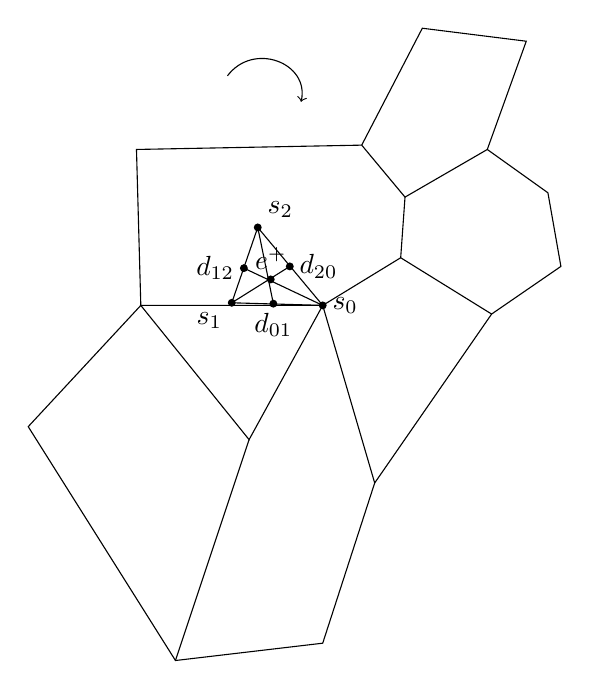
\begin{tikzpicture}[scale=1.1]
\coordinate (a) at (-1.5,0);\coordinate (b) at (.6,0);
\coordinate (c) at (1.5,.55);\coordinate (d) at (1.55,1.25);
\coordinate (e) at (1.05,1.85);\coordinate (f) at (-1.55,1.8);
\draw (a)--(b)--(c)--(d)--(e)--(f)--cycle;
\draw (e)--(1.75,3.2)--(2.95,3.05)--(2.5,1.8)--(d);
\draw (2.5,1.8)--(3.2,1.3)--(3.35,.45)--(2.55,-.1)--(c);
\draw (a)--(-.25,-1.55)--(b)--(1.2,-2.05)--(2.55,-.1);
\draw (a)--(-2.8,-1.4)--(-1.1,-4.1)--(.6,-3.9)--(1.2,-2.05);
\draw (-.25,-1.55)--(-1.1,-4.1);
\draw[->] (-.5,2.65) .. controls (-.2,3.05) and (.45,2.8) .. (.35,2.35);
\coordinate (s1) at (-.45,.03);\coordinate (s2) at (-.15,.9);\coordinate (s0) at (.6,0);
\coordinate (d12) at (-.31,.43);\coordinate (d20) at (.22,.45);\coordinate (d01) at (.03,.02);\coordinate (ep) at (0,.3);
\draw (s1)--(s2)--(s0)--cycle;
\draw (s1)--(d20) (s2)--(d01) (s0)--(d12);
\foreach \p in {s1,s2,s0,d12,d20,d01,ep}{\fill (\p) circle (1.3pt);}
\node[below left] at (s1) {$s_1$};\node[above right] at (s2) {$s_2$};\node[right] at (s0) {$s_0$};
\node[left] at (d12) {$d_{12}$};\node[right] at (d20) {$d_{20}$};\node[below] at (d01) {$d_{01}$};\node[above] at (ep) {$e^+$};
\end{tikzpicture}}

\figure{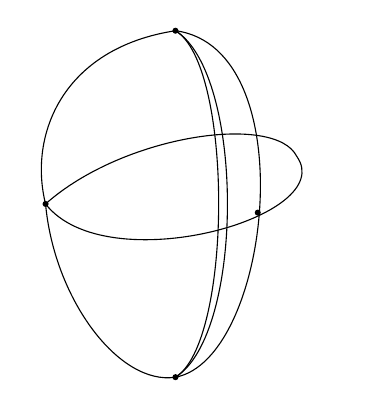
\begin{tikzpicture}[scale=1.1]
\draw (0,2) .. controls (-1.3,1.8) and (-1.7,.8) .. (-1.5,0)
 .. controls (-1.4,-1.1) and (-.65,-2.1) .. (0,-2)
 .. controls (1.1,-1.8) and (1.5,1.8) .. (0,2);
\draw (0,2) .. controls (.8,1.5) and (.8,-1.5) .. (0,-2);
\draw (0,2) .. controls (.67,1.6) and (.66,-1.6) .. (0,-2);
\draw (-1.5,0) .. controls (-.6,.8) and (1.15,1.05) .. (1.4,.55) .. controls (1.9,-.15) and (-.8,-.9) .. (-1.5,0);
\fill (0,2) circle (1pt);\fill (0,-2) circle (1pt);
\fill (-1.5,0) circle (1pt);\fill (.95,-.1) circle (1pt);
\end{tikzpicture}}
\diagram{\begin{tikzcd}[ampersand replacement=\&]
\mathbb P^1_{\overline{\mathbb Q}} \& \mathbb P^1_{\overline{\mathbb Q}}\arrow[l,"\varphi"']
\end{tikzcd}}
\figure{\begin{tikzpicture}[scale=2]
\draw (-1.08,0)--(2.45,0);\draw (.5,-1.4)--(.5,1.8);
\draw (0,0) circle (1);\draw (1,0) circle (1);
\draw[gray,thin] (-1,.02) .. controls (-.95,.9) and (-.2,1.22) .. (.5,.866)
 .. controls (1.15,1.25) and (1.9,.9) .. (2,.02);
\draw[gray,thin] (0,-.03) .. controls (.05,-.7) and (.3,-.86) .. (.5,-.866)
 .. controls (1.1,-1.15) and (1.8,-.9) .. (2,-.03);
\foreach \x in {-1,0,.5,1,2}{\draw (\x,-.025)--(\x,.025);}
\node[below] at (-1,-.03) {$-1$};\node[below] at (0,-.03) {$0$};
\node[below] at (.5,-.03) {$\tfrac12$};\node[below] at (1,-.03) {$1$};\node[below] at (2,-.03) {$2$};
\node[above right] at (.5,.866) {$-j$};
\fill (.5,-.866) circle (.9pt);\node[right] at (.5,-.866) {$-\bar j$};
\end{tikzpicture}}

\scanpage{80}
% archive foliation: 79
Groupe profini \uline{spécial}

\unsure{1} C'est un système \inserted{$\Sigma=$}
$(T,\pi,I,(\Phi_i)_{i\in I}\in(\operatorname{Homext}(T,\pi))^I)$
avec
\[
\Sigma\left\{\begin{array}{l}
T\ \text{groupe profini}\ \simeq\widehat{\mathbb Z}\\
\pi\ \text{groupe profini}\\
I\ \text{ensemble fini}\\
\Phi_i\in\operatorname{Homext}(T,\pi)\qquad\text{pour }i\in I
\end{array}\right.
\]
avec l'axiome que ce système est \deleted{\unsure{spécial}}\inserted{isomorphe}
à l'un des systèmes $\Sigma_\nu$ ($\nu\in\mathbb N$, $\nu\geq1$)
suivants :
\[
\Sigma_\nu\left\{\begin{array}{l}
T=\widehat{\mathbb Z}\\
\pi=\text{groupe profini }\inserted{\pi_\nu=}\widehat L_\nu,\quad
\text{où }L_\nu=\{\lambda_0,\ldots,\lambda_\nu\mid\lambda_0\lambda_1\cdots\lambda_\nu=\unsure{1}\}\\
\qquad(\text{donc }\pi\text{ prolibre à }\nu\text{ générateurs})\\
\unsure{\Phi|I}=[0,\nu]_{\mathbb N}\\
\Phi_i=\text{classe de l'hom }\widehat{\mathbb Z}\xrightarrow{\varphi_i}\pi
\quad\text{tel que }\varphi_i(1)=\lambda_i
\end{array}\right.
\]
\uline{NB} $I$ peut être interprété comme une \uline{partie} de $\operatorname{Homext}(T,\pi)$.
Si $\Sigma\simeq\Sigma_\nu$, $\nu$ est uniquement déterminé
comme $\operatorname{card}I-1$, ou \deleted{\unsure{le}}
\deleted{\unsure{le rang}}, comme rang profini de $\pi_{\mathrm{ab}}$. Pour
$\nu$ fixé, la catégorie des $\Sigma$ correspondants
est équivalente à la catégorie des torseurs
sous
\[
\widetilde A_\nu=\operatorname{Aut}(\Sigma_\nu)
\]
On a des homomorphismes
\[
\widetilde A_\nu\longrightarrow\unsure{\mathfrak S|\mathcal S}_{\nu+1}
\quad(=\operatorname{Aut}(I_\nu))
\]
\[
\widetilde A_\nu\xrightarrow{\chi}\operatorname{Aut}\widehat{\mathbb Z}
\simeq\widehat{\mathbb Z}^{*}
\]

\scanpage{81}
% archive foliation: 80
donnant naissance à
\[
\widetilde A_\nu\longrightarrow\unsure{\mathfrak S|\mathcal S}_{\nu+1}\times\widehat{\mathbb Z}^{*}
\]
qui est \uline{surjectif}. Le noyau de $\widetilde A_\nu\to\unsure{\mathfrak S|\mathcal S}_{\nu+1}$
est noté $A_\nu$, celui de $\widetilde A_\nu\to\unsure{\mathfrak S|\mathcal S}_{\nu+1}\times\widehat{\mathbb Z}^{*}$
est noté $A_\nu^\circ$. D'ailleurs on a
un homomorphisme injectif
\[
\pi\longrightarrow A_\nu^\circ\subset A_\nu
\]
via automorphismes intérieurs. Le conoyau
\inserted{de $\pi\to A_\nu^\circ$ ($\pi\to A_\nu$, $\pi\to\widetilde A_\nu$)}
se \deleted{\unsure{on}} note $\Gamma_\nu^\circ$ \inserted{($\Gamma_\nu$, $\widetilde\Gamma_\nu$)}, d'où on a des
suites exactes
\diagram{\ensuremath{\left\{\begin{array}{l}
1-\pi\longrightarrow A_\nu^\circ\longrightarrow\Gamma_\nu\longrightarrow1\\
\deleted{\unsure{1-\pi-}}\\
1\longrightarrow A_\nu\longrightarrow\widetilde A_\nu\longrightarrow\unsure{\mathfrak S|\mathcal S}_{\nu+1}-1
\end{array}\right.}}
\[
1\unsure{\Longrightarrow|\longrightarrow} A_\nu^\circ\longrightarrow A_\nu-\widehat{\mathbb Z}^{*}-1
\]
\[
\overbrace{\pi\quad\Gamma_\nu^\circ\quad\widehat{\mathbb Z}^{*}\quad\unsure{\mathfrak S|\mathcal S}_{\nu+1}}^{\widetilde A^{\unsure{\nu|\vphantom{\nu}}}}
\qquad\text{filtration}
\]
\uline{Exemples} \textcircled{I} Soit $X$ droite projective sur
$k$ alg. clos de car. $0$, $I\subset X(k)$, $\operatorname{card}I=\nu+1$
\[
T=\unsure{T_{\bullet}}(k)=\varprojlim_n\mu_n(k),\qquad
\pi=\pi_1(X\setminus I,x)
\]
où $x\in X(k)-I$. Il \deleted{\unsure{que}} y a par Kummer

\scanpage{82}
% archive foliation: 81
des $\Phi_i\in\operatorname{Homext}(T,\pi)$ canoniques,
$i\in I$. Le système
\deleted{$\unsure{\Sigma(X/I/k)}$}\inserted{$\Sigma(X/I/x/k)$}$=(T,I,\pi,(\Phi_i))$
satisfait aux conditions \unsure{envisag.} \deleted{Pour}
\inserted{Au lieu de} \deleted{\unsure{Changeons}} \deleted{\unsure{le}} prendre $x$, il suffit
de prendre un $\unsure{\xi|\zeta}$, foncteur fibre sur
la catégorie des rev. étales de $X\setminus I$
($\pi$ étant le groupe des autom. de $\xi\ldots$)
Alors $\Sigma$ dépend fonctoriellement de
$(X/I/\xi/k)$. Prenant $X,I,k$ fixes,
$\xi$ variable, on voit que $\Sigma$ est déterminé
``mod autom. intérieurs'' i.e. \deleted{\unsure{on est}}
définit un torseur \deleted{sous}\inserted{à droite} \unsure{non pas}
sous $\widetilde A_\nu$ mais sous son quotient
$\widetilde A_\nu/\pi_\nu=)\ \widetilde\Gamma_\nu$,
\inserted{soit $P(X/I/k)$}, \deleted{le dernier torseur}
dont le commutant est le groupe
des ``autom. ext.'' de \deleted{$\unsure{T,I,}$}
$\Sigma(X/I/\unsure{x|m}/k)\ldots$

Supposons que $X/I/\unsure{x}$ provienne
par extension de la base \deleted{$\unsure{\operatorname{Spec}k\longrightarrow S_0}$}\inserted{$k_0\subset k$}
\deleted{d'une situation}

\scanpage{83}
% archive foliation: 82
\deleted{$\unsure{X_0/S}$} d'une situation $X_0/I_0/\unsure{x_0|k_0}/k_0$
où $k_0$ est un sous-corps. [OPS \unsure{disons} que
$k$ est une clôture alg. de $k_0\ldots$].
Alors $\Gamma=\operatorname{Gal}(\overset{\unsure{\longleftarrow|\longleftrightarrow}}{k/k_0})$ opère sur
$\Sigma^{\mathrm{ext}}$ par transport de structure, donc on a
une \deleted{\unsure{la}} opération aussi sur $P(X/I/k)$,
\deleted{donc}\inserted{ou encore} un hom
\[
\Gamma\longrightarrow{}^{P(X/I/k)}\widetilde\Gamma_\nu
\simeq\operatorname{Aut}(\Sigma^{\mathrm{ext}})
\]
qui par image inverse \inserted{d'extensions} donne naissance
à l'extension
\[
1-\pi_1(X\setminus I,x)-\pi_1(X_0\setminus I_0,x_0)
\longrightarrow\pi_1(k_0/k)-1
\]
$\ldots\quad\Gamma\xrightarrow{\chi}\operatorname{Aut}(T)\simeq\widehat{\mathbb Z}^{*}$
est l'hom de Kummer-Tate $\ldots$

\textcircled{II} \uline{Plus} précisément supposons $k_0=\mathbb Q$, $X_0=\mathbb P^1_{\mathbb Q}$,
\inserted{$\overline{\mathbb Q}$ clôture alg. de $\mathbb Q$ dans $\mathbb C$},
\[
I=\mu_{\nu+1}(\overline{\mathbb Q})=\mu_{\nu+1}(\mathbb C^{*})
\subset\overline{\mathbb Q}
=\unsure{\mathbb E|\mathbb A}^1_{\overline{\mathbb Q}}(\overline{\mathbb Q})
\subset\mathbb P^1_{\overline{\mathbb Q}}(\overline{\mathbb Q})
\]
On trouve un isomorphisme canonique,
via l'exponentielle et les lacets
\deleted{$\unsure{I\simeq[0,\nu]|I\simeq[0,1]}$},
\[
\Sigma(X/I/k)^{\mathrm{ext}}\simeq L_\nu^{\mathrm{ext}}
\]
donc $P(X,I/k)=$ torseur trivial

\scanpage{84}
% archive foliation: 83
d'où
\[
\Gamma=\operatorname{Gal}(\overline{\mathbb Q}/\mathbb Q)
\longrightarrow\widetilde{\mathcal T}_\nu
\]
L'hom correspondant
\[
\Gamma\longrightarrow\unsure{\mathfrak S|\mathcal S}_{\nu+1}
\]
se fait via
\[
\Gamma\longrightarrow\mu_{\nu+1}(\mathbb C^{*})\simeq\mathbb Z/\nu+1
\xrightarrow{\mathrm{can}}\unsure{\mathfrak S|\mathcal S}_{\nu+1}\ldots
\]
L'intérêt de prendre $I$ comme
dessus est d'avoir une opération
de \inserted{$\mathbb Z/2\cdot$}$\mu_{n\,\mathbb Q}$ \deleted{\unsure{trans.}} sur la situation
$(X_0/I_0/\mathbb Q)$ donc de \inserted{$\mathbb Z/2\cdot$}$\mu_n(\overline{\mathbb Q})\ (=D_n)$
sur $X/I/\mathbb Q$ --- en fait, le
produit $\tfrac12$ direct
$(\Gamma\times\deleted{\unsure{\mathbb Z/2}})\underbrace{\mu_n(\overline{\mathbb Q})}_{\subset\overline{\mathbb Q}^{*}}$\unsure{$=$}
opère sur $X/I/\overline{\mathbb Q}$ donc
\deleted{s'envoie dans}
\[
(\Gamma\times\mathbb Z/2)\cdot\mu_n(\overline{\mathbb Q})
\unsure{\longrightarrow|\Longrightarrow}
\widetilde{\mathcal T}_\nu
\]
où l'hom $\mu_n(\overline{\mathbb Q})\longrightarrow\widetilde{\mathcal T}_\nu$
\margin{$n=\nu+1$}

\scanpage{85}
% archive foliation: 84
se déduit de l'hom évident
\[
\mu_n(\overline{\mathbb Q})\xrightarrow{\rho_\nu}\widetilde A_\nu
\]
provenant de la permutation circulaire des
gén. de $\widehat L_\nu$ --- l'opération de
$\mathbb Z/2$ dans $\widetilde{\mathcal T}_\nu$ provient de $=$ de
l'opération
\[
\mathbb Z/2-\widetilde A_\nu
\]
\deleted{\unsure{par}}
\[
\left\{\begin{aligned}
(\lambda_0,\lambda_1,\ldots,\lambda_\nu)&\xrightarrow{t_\nu}
\deleted{(\unsure{\lambda_0},\lambda_\nu,\lambda_{\nu-1},\ldots,\lambda_1)}\\
&\inserted{(\lambda_0,q_\nu\lambda_\nu q_\nu^{-1},
q_{\nu-1}\lambda_{\nu-1}q_{\nu-1}^{-1},\ldots,
\unsure{q_2}\lambda_2q_2^{-1},\lambda_1)}\\
&\text{où }\unsure{q_i|g_i}=\lambda_{\unsure{0|1}}\cdots\lambda_{i-1}
\end{aligned}\right.
\]
qui renverse l'ordre circulaire.
\margin{\uline{vérifier ?}}
Ceci dit donc que l'hom
\diagram{\begin{tikzcd}[ampersand replacement=\&,column sep=large]
\Gamma\arrow[r,"i_\nu"]\&\widetilde{\mathcal T}_\nu\arrow[r,dotted,dash,"\varepsilon_\nu"]\&\unsure{\mathfrak S|\mathcal S}_n\supset(\mathbb Z/n)^*
\end{tikzcd}}
\deleted{$\unsure{\mu_n(\overline{\mathbb Q})}$}
satisfait, en plus de
\[
\left[\varepsilon_\nu i_\nu=\chi_n\right.\quad\unsure{aux|ou}
\]
la relation
\[
\left\{\begin{aligned}
&i_\nu(\Gamma)\text{ commute à }t_\nu\\
&i_\nu(\gamma)\rho_\nu(i)\unsure{i_\nu|t_\nu}(\gamma)^{-1}
=\rho_\nu(\chi_n(\gamma)i)
\end{aligned}\right.
\]

\scanpage{86}
% archive foliation: 85
Soit $\mathcal T_\nu^!$ le ss-groupe de $\mathcal T_\nu$
formé des éléments qui satisfont
aux relations précédentes. Donc on a
\[
1\longrightarrow\mathcal T_\nu^{!0}\unsure{-|\longrightarrow}\mathcal T_\nu^!\longrightarrow\widehat{\mathbb Z}^{*}\unsure{-|\longrightarrow}1
\]
avec
\[
\begin{gathered}
\mathcal T_\nu^{!0}\subset\mathcal T_\nu^0\\
\text{''}\\
\{\gamma\in\mathcal T_\nu^0\mid\gamma\text{ commute aux }\rho_\nu(i)
\text{ et à }t_\nu\}
\end{gathered}
\]
\figure{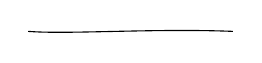
\begin{tikzpicture}\draw (0,0)..controls (.5,-.04) and (1.6,.04)..(2.6,0);\end{tikzpicture}}

Si $\nu=2$ il y a un autre choix
intéressant de $I_{\unsure{0}}\subset\mathbb P^1(\overline{\mathbb Q})$, savoir
\[
I=\{0,1,\infty\}\qquad(\text{plutôt que }I=\mu_3(\overline{\mathbb Q}))
\]
qui donne lieu à action de
$\unsure{\mathfrak S|\mathcal S}_3$ sur $(X_0/I_0/k)$ --- on trouve
action de $\Gamma\times\unsure{\mathfrak S|\mathcal S}_3$ sur $\unsure{F_2|\Gamma_2}^{\mathrm{ext}}$, i.e.
\[
\Gamma\times\unsure{\mathfrak S|\mathcal S}_3\longrightarrow\widetilde{\mathcal T}_2
\]

\scanpage{87}
% archive foliation: 86
En fait on a ici, exceptionnellement
\[
\widetilde{\mathcal T}_2\simeq\unsure{\mathfrak S|\mathcal S}_3\cdot\mathcal T_2
\]
(produit $\tfrac12$ direct pour action de $\unsure{\mathfrak S|\mathcal S}_3$ sur $\mathcal T_2$)
\[
\Gamma\longrightarrow\deleted{\unsure{\mathcal T_2|\widetilde{\mathcal T}_2}}\ \widetilde{\mathcal T}_2
\overset{\varepsilon}{-}\unsure{\mathfrak S|\mathcal S}_3\qquad\text{trivial}
\]
i.e. $\Gamma\longrightarrow\deleted{\unsure{\mathfrak S|\mathcal S}_3}\ \unsure{\widetilde{\mathcal T}_2|\mathcal T_2}$, d'où
\[
\boxed{\Gamma\longrightarrow\mathcal T_2^{\unsure{\mathfrak S|\mathcal S}_3}}
\]
On aurait envie de définir un
iso can. $\mathcal T_2^!\simeq\mathcal T_2^{\unsure{\mathfrak S|\mathcal S}_3}$
\margin{?}
et des iso can
\[
\mathcal T_2^!\simeq\mathcal T_\nu^!
\]
Pour ceci, on va généraliser d'

\scanpage{89}
% archive foliation: 88
\uline{Groupes prolibres} spéciaux.
\[
\left\{\begin{array}{l}
\pi\ \text{groupe profini}\\
\unsure{T|L}\quad\widehat{\mathbb Z}\text{-Module libre}
\deleted{\simeq\widehat{\mathbb Z}\text{ (isomorphisme non précisé)}}\inserted{\text{de rang }1}\\
\Phi_i\in\operatorname{Homext}(L,\pi)\deleted{\unsure{\Phi}}
\qquad0\leq i\leq\nu\qquad(\nu\geq2)
\end{array}\right.
\]
\uuline{Hyp} :
\[
\left\{\begin{array}{l}
\exists\ e\in\unsure{T|L}^*\quad(\text{base de }L)\\
(\varphi_i)_{0\leq i\leq\nu}\in\displaystyle\prod_{0\leq i\leq\nu}\Phi_i
\end{array}\right|\ \text{tels que, posant }h_i=\varphi_i(e),
\]
l'hom de
\diagram{\begin{tikzcd}[ampersand replacement=\&]
\inserted{\widehat L_\nu}\deleted{\unsure{\widehat F([0,\nu])}}\arrow[r]\&\pi\\
\lambda_i\arrow[r,mapsto]\&h_i
\end{tikzcd}}
\inserted{groupe prolibre \deleted{sur $[0,\nu]$}
engendré par $\lambda_0,\ldots,\lambda_\nu$ avec $\lambda_0\cdots\lambda_\nu=1$}
soit un \uline{isomorphisme}

En d'autres termes
Soit $\pi_0$ \inserted{$=\widehat L_\nu=$} \deleted{groupe pro.}
$(\lambda_0,\ldots,\lambda_\nu\mid\lambda_0\lambda_1\cdots\lambda_\nu=1)^{\wedge}$
\[
T_0=\widehat{\mathbb Z},\quad e_0=1
\]
$\Phi_{0i}$ classe de
\diagram{\begin{tikzcd}[ampersand replacement=\&]
\widehat{\mathbb Z}\arrow[r]\&\pi_\nu\\
e_0\arrow[r,mapsto]\&\lambda_i
\end{tikzcd}}
on veut que $(\pi,T,(\Phi_i))$ soit isom. à $(\pi_0,T_0,(\Phi_{0i}))$
\[
A_\nu=\operatorname{Aut}(\widehat L_\nu,T_0,(\Phi_{0i}))
\xrightarrow{\chi_\nu}\widehat{\mathbb Z}^{*}
\underset{\operatorname{Aut}(T_0)}{\text{''}}
\]
on \unsure{prouve} que c'est surjectif
\[
\widehat L_\nu\xrightarrow{i}\deleted{\unsure{A.}}\operatorname{Ker}\chi_\nu\subset A_\nu
\qquad\text{injectif}
\]
\[
g\longmapsto(\operatorname{int}(g),\operatorname{id}_{T_0})
\]
\[
u\,i(g)\,u^{-1}=i(u(g))
\]
i.e. $\widehat L_\nu$ invariant ds $A_\nu$
\[
A_\nu/\widehat L_\nu=\Gamma_\nu
\]
on veut élucider sa structure.
